\chapter{Blockchain}

Cryptocurrencies, since 2008\footnote{Year of Bitcoin's whitepaper by Sathosi Nakamoto.} has received a lot of consideration from whom is interested into investing or building products and services for a self-interest income but also has gained attentions on the underlying technology on which all cryptocurrencies are based on: \textbf{blockchain}.\newline
\newline
There isn't a globally accepted definition of \textit{Blockchain} due to different implementations and flavours but is possibile to delineate some key points.\newline
A blockchain is a \textbf{fully-distributed}, \textbf{peer-to-peer network} which makes use of \textbf{cryptography} to \textbf{securely} host applications, store data and transfer digital assets; this technology can be thought as an \textbf{append-only} master ledger that is \textbf{publicly available} and is not controlled by a \textbf{central authority}.

This definition is interesting since do not mention financial or particular use cases and do not specificy consensus protocols or algorithms due to the fact that blockchain's technology can be implemented to be a general purpose system and not only a mechanism to achieve electronic payments; in fact the first ever known blockchain was designed by two cryptographers in 1991: \textit{Stuart Haber} and \textit{Scott Stornetta} to digitally time-stamps documents and prevents data tampering and authentication.

\section{History}

The first modern blockchain using an anonymous, distributed and cryptographic payments system is the Bitcoin's blockchain that was presented by Sathosi Nakamoto in 2008 to solve the problem of building and using a decentralized protocol to implement digital currency without the need of a trusted authority or central server and avoid double-spending from malicious players.\newline
A lot of others proposal were made before Bitcoins but they do not fully solved the problems of decentralization and consensus and were used as bases for new blockchain technologies.\newline\newline
The first known blockchain is not the one implemented in Bitcoin's project because in 1991, cryptographers \textit{Stuart Haber} and \textit{Scott Stornetta}, wanted to implement a system where documents time-stamps could not be tampered\cite{haberstorneta}.

\subsection{Haber and Stornetta blockchain's}

Stornetta and Haber's idea was to certify the date a document was created or modified; for example, in intellectual property matters, it is sometimes crucial to verify the date of an inventor first patentable prototype; the solution requires to solve two problems:

\begin{enumerate}
    \item the data itself should be time-stamped (not the medium);
    \item impossibility of changing the time-stamp.
\end{enumerate}

The solution proposed can achieve digital time-stamping of such documents so that it is infeasible for an attacker to alter the date.\newline
The process of time-stamping a document can be solved using a family of cryptographically secure \textit{collision-free} hash functions $h: \{0,1\}^* -> \{0,1\}^l$. Those functions $h$ are easy to compute but it is computionally infeasible to find a $x^1$ such that $h(x)=h(x^1), \forall x,x^1: x \neq x^1$ (\textit{strong collision resistance})\footnote{Weak collision resistance or \textit{second preimage resistance} is optional since the solution requires that two distinct preimages hash to the same value.}.\\

\begin{figure}
    \centering
    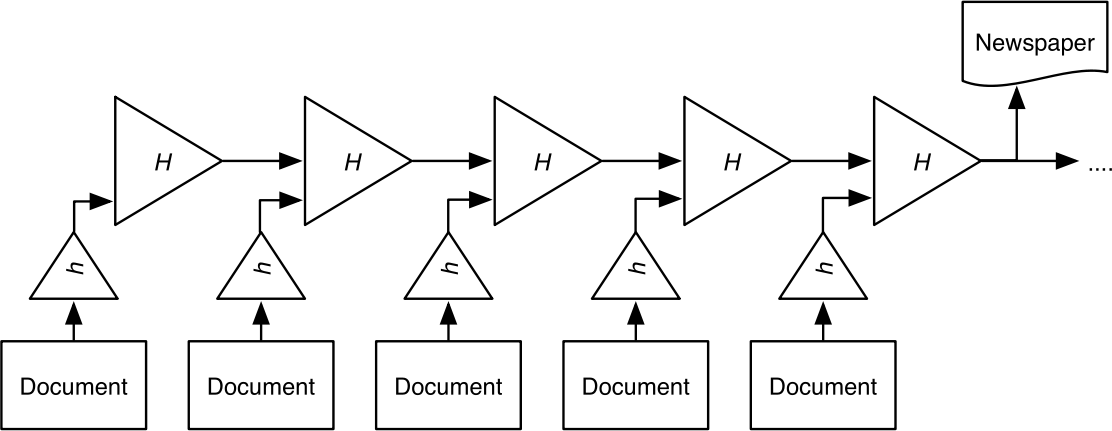
\includegraphics[scale=1.2]{images/haberstornetta.png}
\end{figure}

Using hash functions is also possibile to avoid providing the entire document to some time-stamping service and thus the privacy is guaranteed: for example the content of an intellectual property is not disclosed.\newline\newline
Once the hash of the document is calculated is possibile to generate a digital signature to identify the signer: for example is possible to appends the date, time and sign to the new compound document.

The first solution proposed used a third party service (\textit{Time-Stamping Service}) to elaborate and sign the documents but the TSS service can issue false time-stamps: it is necessary to implement a solution in the absence of generally trusted parties.

Two possibile solutions can be used or combined:

\begin{itemize}
    \item Use a possible untrustworthy TSS service constrained to produce genuine time-stamps in a way that false ones are difficult to generate using \textit{linking};
    \item Distribute the required trust among the users of the service (\textit{decentralization}).
\end{itemize}

In the first, the hashes, of documents submitted are linked togheter and certificates recording the linking of a given document are distributed to other clients both upstream and downstream from that document.\newline
In the second solution, several clients are randomly choosen to time-stamp the hash.

A practical implementation of Haber and Stornetta blockchain has been running since 1995: \textit{Surety}\footnote{\url{http://surety.com/}} company every week publish a \textit{base 16} string of the hash of all new signatures of their clients over the week on the \textit{New York Times} journal.\\

\begin{figure}[!h]
    \centering
    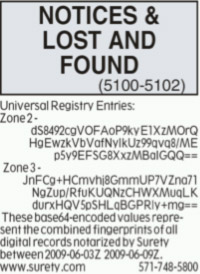
\includegraphics[scale=0.5]{images/nyt.jpg}
    \caption{\textit{Base 16} of the hash Surety published on New York Times.}
    \source{Surety}
\end{figure}

\subsection{Blockchain as payment system}

The theoric implementation of Haber and Stornetta blockchain is very similar to the one presented in the Bitcoin Whitepaper \textit{Bitcoin: A Peer-to-Peer Electronic Cash System}\cite{bitcoin} since it was a solid technological platform used by Satoshi Nakamoto; in fact three of heights papers cited in Bitcoin's whitepaper were written by \textit{Haber} and \textit{Stornetta}.

Banks should keep track of all parties balances in a ledger that is not visible by the public. Banks system rely on trust: each party should trust the bank upon every transaction and the bank can decide to reject or accept it.\\
This centralization is the first aspect that lead to the implementation of firsts electronic payments based on cryptography techniques in 1990s and early 2000s: \textit{eCash}, \textit{SET}, \textit{Hashcash} and \textit{b-cash}.


\section{Structure}

Technically speaking a blockchain is a grown list of records, called blocks, which are linked using cryptographic techniques and widely used by cryptocurrencies.\\
There is no actually a formal definition of blockchain technology that is generally accepted but is possible to defined it using the Bitcoin as model and its application in cryptocurrencies.\\

A blockchain is commonly composed in:
\begin{itemize}
    \item Blocks
    \item Protocols
    \item Nodes
\end{itemize}

\subsection{Blocks}

A block in a single record that forms the growing list of records.

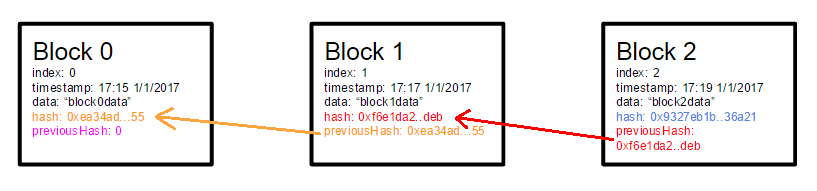
\includegraphics[scale=0.45]{images/blockchain_basic.png}

Blocks are linked using cryptography and by design are resistant to data modification. Cryptography provides authentication and verification and is used to conjure a secure computing environment out of many nodes without central authority or single owner.\\
Each block contains a cryptographic hash of the previous block, a timestap and the data to store in a permanent way.

Each block contains a cryptographic hash of the previous block,[6] a timestamp, and transaction data (generally represented as a merkle tree root hash). By design, a blockchain is resistant to modification of the data. It is "an open, distributed ledger that can record transactions between two parties efficiently and in a verifiable and permanent way".[8] For use as a distributed ledger, a blockchain is typically managed by a peer-to-peer network collectively adhering to a protocol for inter-node communication and validating new blocks. Once recorded, the data in any given block cannot be altered retroactively without alteration of all subsequent blocks, which requires consensus of the network majority.

Though blockchain records are not unalterable, blockchains may be considered secure by design and exemplify a distributed computing system with high Byzantine fault tolerance. Decentralized consensus has therefore been claimed with a blockchain.[9]

Blockchain was invented by Satoshi Nakamoto in 2008 to serve as the public transaction ledger of the cryptocurrency bitcoin.[1] The invention of the blockchain for bitcoin made it the first digital currency to solve the double-spending problem without the need of a trusted authority or central server. The bitcoin design has inspired other applications.[1][3]
Qui una breve descrizione del contenuto del capitolo o, eventualmente, testo introduttivo alle sezioni che seguono

\section{Prima Sezione}
Qui il testo della prima sezione. Questa è  una parola in \textit{corsivo}, questa invece è una parola in \textbf{grassetto} e questa è una parola in \texttt{monotype}.

\begin{center}
Questo è un paragrafo centrato!
\end{center}

Dimensione del testo:\\

\LARGE{Testo} \Large{Testo} \large{Testo} \normalsize{Testo} \small{Testo} \footnotesize{Testo}\\

Qui una citazione bibliografica \cite{bib001}.

Qui un link \url{www.google.it}


\subsection{Prima Sottosezione}

Qui l'esempio di un elenco puntato:

\begin{itemize}
\item Primo elemento,
\item Secondo elemento,
\item Terzo elemento.
\end{itemize}

Qui l'esempio di un elenco con un sotto-elenco:

\begin{itemize}
\item Primo elemento,
\begin{itemize}
\item Primo elemento del sotto-elenco
\item Secondo elemento del sotto-elenco
\end{itemize}
\item Secondo elemento,
\item Terzo elemento.
\end{itemize}

Qui infine l'esempio di un elenco numerato

\begin{enumerate}
\item Testo
\item Testo
\item Testo
\end{enumerate}

\section{Seconda Sezione}\label{sec:Sezione2}

Qui l'esempio di una formula matematica:

$ G = \gamma\dfrac{m_{1}m_{2}}{r^{2}} $

\section{Terza Sezione}

Qui il riferimento ad una sezione utilizzando una label: Sezione \ref{sec:Sezione2}

Qui la definizione di due paragrafi con titoli.

\paragraph{Titolo 1} testo del paragrafo

\paragraph{Titolo 2} testo del paragrafo, con una nota a piè di pagina\footnote{Questo è il testo della nota, in cui si può \textit{utilizzare} qualunque stile di \textbf{formattazione}}

% NeoTex: mainfile=main.tex:


\chapter{Capitolo con Immagini e Codice}

Introduzione al capitolo

\section{Prima sezione del secondo capitolo}

Qui di seguito un'immagine. Tutte le immagini devono essere inserite nella cartella \texttt{images}

\begin{figure}[H]
\centering

\includegraphics[scale=0.8]{images/placeholder.jpg}
\caption{Testo della didascalia}
\label{fig:figure1}
\end{figure}

Qui invece il testo con il riferimento all'immagine: Figura \ref{fig:figure1}.

Qui un'immagine con due sotto-immagini:

\begin{figure}[H]
\centering
\begin{subfigure}[b]{0.42\textwidth}

\includegraphics[width=\textwidth]{images/placeholder.jpg}
\caption{Didascalia prima figura}
\label{fig:figure2}
\end{subfigure}
\qquad
\begin{subfigure}[b]{0.42\textwidth}

\includegraphics[width=\textwidth]{images/placeholder.jpg}
\caption{Didascalia seconda figura}
\label{fig:figure3}
\end{subfigure}
\caption{Didascalia globale}
\label{fig:figures12}
\end{figure}

Altri tipi di riferimenti: Figura \ref{fig:figures12} oppure \ref{fig:figure3}.

\section{Seconda sezione con codice sorgente}

Il codice sorgente può essere inserito mediante un link al file del codice sorgente, in questo caso il file con il codice va inserito nella cartella \texttt{code}.
